%\documentclass[10pt,aspectratio=43,t,l]{beamer}
\documentclass[10pt,aspectratio=169,t,l,fleqn,mathsanserif,sanserif]{beamer}
%\documentclass[10pt]{beamer}

%\setbeamertemplate{footline}[page number]{}

\usepackage{framed}
\usepackage{tcolorbox}
\colorlet{shadecolor}{blue!15}
\usepackage{color,amsmath,xmpmulti,textpos,comment,eurosym,bm,amsthm,tabularx,cancel}
\usepackage{epsfig}
\usepackage{nicefrac}
\usepackage{listings}
%\usepackage{enumitem}
\usepackage{graphicx}    
\usepackage{graphics}
\usepackage{epstopdf}
\usepackage[normalem]{ulem}
\usepackage{float}
%\usepackage[cmbold]{mathtime}
%\usepackage{mt11p}
\usepackage{placeins}
\usepackage{amsmath}
\usepackage{pifont}
\usepackage{color}
\usepackage{amssymb}
\usepackage{mathtools}
\usepackage{subfigure}
\usepackage{multirow}
\usepackage{epsfig}
\usepackage{listings}
%\usepackage{enumitem}
\usepackage{rotating,tabularx}
%\usepackage[graphicx]{realboxes}
\usepackage{graphicx}
\usepackage{graphics}
\usepackage{epstopdf}
\usepackage{longtable}
%\usepackage[pdftex]{hyperref}
\usepackage{breakurl}
\usepackage{epigraph}
\usepackage{xspace}
\usepackage{amsfonts}
\usepackage{eurosym}
\usepackage{ulem}
\usepackage{footmisc}
\usepackage{comment}
\usepackage{setspace}
\usepackage{geometry}
\usepackage{caption}
\usepackage{pdflscape}
\usepackage{array}
\usepackage[round]{natbib}
\usepackage{booktabs}
\usepackage{dcolumn}
\usepackage{mathrsfs}
\usepackage{tikz}
\usetikzlibrary{decorations.pathreplacing}
\usepackage{sansmathaccent}
\pdfmapfile{+sansmathaccent.map}
\usetikzlibrary{shapes.geometric, arrows,chains}
\tikzset{
  startstop/.style={
    rectangle, 
    rounded corners,
    minimum width=3cm, 
    minimum height=1cm,
    align=center, 
    draw=black, 
    fill=red!30
    },
  startsleft/.style={
    rectangle, 
    rounded corners,
    minimum width=3cm, 
    minimum height=1cm,
    align=left, 
    draw=black, 
    fill=red!30
    },
  startsright/.style={
    rectangle, 
    rounded corners,
    minimum width=3cm, 
    minimum height=1cm,
    align=right, 
    draw=black, 
    fill=red!30
    },
  process/.style={
    rectangle, 
    minimum width=3cm, 
    minimum height=1cm, 
    align=center, 
    draw=black, 
    fill=blue!30
    },
  decision/.style={
    rectangle, 
    minimum width=3cm, 
    minimum height=1cm, align=center, 
    draw=black, 
    fill=green!30
    },
  arrow/.style={thick,->,>=stealth},
  dec/.style={
    ellipse, 
    align=center, 
    draw=black, 
    fill=green!30
    },
  font={\fontsize{9pt}{12}\selectfont}
}
%\renewcommand{\labelitemi}{$\blacktriangleright$}

\epstopdfsetup{outdir=./}

\newcolumntype{Y}{>{\centering\arraybackslash}X}
\def\Put(#1,#2)#3{\leavevmode\makebox(0,0){\put(#1,#2){#3}}}

\newcommand{\subhead}[1]{\mbox{}\newline\textbf{#1}\newline}
\newcommand{\ave}[1]{\left\langle #1 \right \rangle}
\newcommand{\eg}{{\it e.g.}}
\newcommand{\ie}{{\it i.e.}}
\newcommand{\cf}{{\it c.f.}}
\newcommand{\etc}{{\it etc.}}
\newcommand{\etal}{{\it et al.}}
%\newcommand{\btVFill}{\vskip0pt plus 1filll}

\newcommand{\del}{D}
\newcommand{\hor}{H}


\newcommand{\Ito}{It\^{o}}
\newcommand{\SP}{S{\&}P500}
\newcommand{\lopt}{\ell_{\text{opt}}}
\newcommand{\gest}{g_{\text{N,T}}}
\newcommand{\elabel}[1]{\label{eq:#1}}
\newcommand{\eref}[1]{Eq.~(\ref{eq:#1})}
\newcommand{\Eref}[1]{Equation~(\ref{eq:#1})}

\newcommand{\flabel}[1]{\label{fig:#1}}
\newcommand{\fref}[1]{Fig.~\ref{fig:#1}}
\newcommand{\Fref}[1]{Figure~\ref{fig:#1}}
\newcommand{\person}[1]{{#1}}
\newcommand{\ra}[1]{\renewcommand{\arraystretch}{#1}}
\newcommand{\vs}[1]{\vspace{.#1cm}}
\newcommand{\vf}{\vspace{.25cm}}
\newcommand{\vff}{\vspace{.6cm}}
\newcommand{\np}{\\ \vf}
\newcommand{\npp}{\\ \vff}
\newcommand{\be}{\begin{equation*}}
\newcommand{\ee}{\end{equation*}}
\newcommand{\bea}{\begin{eqnarray*}}
\newcommand{\eea}{\end{eqnarray*}}
\newcommand{\bc}{\begin{center}}
\newcommand{\ec}{\end{center}}
\newcommand{\bie}{\begin{enumerate}}
\newcommand{\eie}{\end{enumerate}}
\newcommand{\bi}{\begin{itemize}}
\newcommand{\ei}{\end{itemize}}
\newcommand{\toinf}{\rightarrow\infty}
\newcommand{\D}{{\Delta}}
\newcommand{\Dx}{{\Delta x}}
\newcommand{\Dy}{{\Delta y}}
\newcommand{\Du}{{\Delta u}}
\newcommand{\DW}{{\Delta W}}
\newcommand{\DU}{{\Delta U}}
\newcommand{\du}{{\delta u}}
\newcommand{\Dv}{{\Delta v}}
\newcommand{\dt}{{\delta t}}
\newcommand{\gens}{g_{\ave{\,}}}
\newcommand{\ft}[1]{\frametitle{#1}}
\newcommand{\bq}{\begin{quote}}
\newcommand{\eq}{\end{quote}}
\newcommand{\ww}[1]{\bq{\small\rm#1\\}\eq}
\newcommand{\E}{\mathrm{E}}
\newcommand{\Var}{\mathrm{Var}}
\newcommand{\Cov}{\mathrm{Cov}}
\newcommand{\sgn}{\mathrm{sgn}}
\newcommand{\prob}[1]{\mathcal{P}\left(#1\right)}
\newcommand{\lra}{\longrightarrow}
\newcommand{\eps}{\varepsilon}
\newcommand{\ga}{g_\text{ave}}
\newcommand{\gt}{g_\text{typ}}
\newcommand{\gbar}{\bar{g}}
\newcommand{\mbar}{\bar{m}}
\newcommand{\red}[1]{\textcolor{red}{#1}}
\newcommand{\xf}{{x_F}}
\newcommand{\xb}{{x_B}}
\newcommand{\muf}{{\mu_F}}
\newcommand{\mub}{{\mu_B}}
\newcommand{\sigf}{{\sigma_F}}
\newcommand{\sigb}{{\sigma_B}}
\newcommand{\gf}{{\gbar_F}}
\newcommand{\gb}{{\gbar_B}}
\newcommand{\pa}{\textit{pa}}
\newcommand{\taus}{{\tau_\text{s}}}
\newcommand{\Dt}{\Delta t}
\newcommand{\etau}{\tau^\text{eqm}}
\newcommand{\taue}{\tau^\text{EGBM}}
\newcommand{\wtau}{\widetilde{\tau}}
\newcommand{\xN}{\ave{x}_N}
\newcommand{\Sdata}{S^{\text{data}}}
\newcommand{\Smodel}{S^{\text{model}}}
\beamertemplatenavigationsymbolsempty

\newcommand{\tlabel}[1]{\label{tab:#1}}
\newcommand{\tref}[1]{Tab.~\ref{tab:#1}}
\newcommand{\Tref}[1]{Table~\ref{tab:#1}}

\newenvironment{myindentpar}[1]%
{\begin{list}{}%
    {\setlength{\leftmargin}{#1}}%
  \item[]%
}
{\end{list}}

%\usetheme[width=1.8cm,hideothersubsections]{Frankfurt}
\usetheme{Frankfurt}

\newcommand\BackgroundPicture[1]{
\setbeamertemplate{background}{
\parbox[c][\paperheight]{\paperwidth}{
\vfill \hfill
\includegraphics[width=1\paperwidth,height=1\paperheight]{#1}
\hfill \vfill
}}}


\definecolor{lmlblue}{RGB}{0,77,123}
\definecolor{deepblue}{RGB}{35,33,169}
\definecolor{lmllb}{RGB}{237,244,255}
\definecolor{lmlred}{RGB}{155,29,29}
\definecolor{lmlgrey}{RGB}{142,142,142}
\definecolor{lmlgrey2}{RGB}{82,82,82}
\definecolor{grey}{RGB}{210,210,210}
\xdefinecolor{lightblue}{rgb}{0,200,255}
\setbeamercolor{important}{bg=lightblue,fg=red}
\AtBeginEnvironment{definition}{%
  \setbeamercolor{block body}{fg=black,bg=white}
  \setbeamercolor{block title}{bg=lmllb,fg=black}
}

\AtBeginEnvironment{theorem}{%
  \setbeamercolor{block body}{fg=black,bg=white}
  \setbeamercolor{block title}{bg=lmllb,fg=black}
}

%\newcommand{\propnumber}{} % initialize
%\newtheorem*{prop}{Proposition \propnumber}
%\newenvironment{propc}[1]
%  {\renewcommand{\propnumber}{#1}%
%   \begin{shaded}\begin{prop}}
%  {\end{prop}\end{shaded}}
%\AtBeginEnvironment{propc}{%
%  \setbeamercolor{block body}{fg=black,bg=white}
%  \setbeamercolor{block title}{bg=lmllb,fg=black}
%}

\setbeamercolor{fine separation line}{fg=lmllb}

\setbeamercolor{item projected}{fg=white, bg=black}

\setbeamercolor{frametitle}{bg=lmllb, fg=black}
\setbeamertemplate{frametitle}[default][left,colsep=-4bp,rounded=false,shadow=false]

\setbeamercolor{structure}{bg=white, fg=black}
%structure changes color of title in sidebar.

%\setbeamertemplate{frametitle}[default][colsep=-4bp,rounded=false,shadow=false]
\setbeamercolor{section in head/foot}{fg=lmlgrey2, bg=lmllb}
\setbeamercolor{normal text}{fg=black}
\setbeamercolor{title}{bg=white,fg=deepblue}

\hypersetup{colorlinks,linkcolor=,urlcolor=deepblue}

\setbeamerfont{title in sidebar}{size=\fontsize{9}{9}\selectfont}
\setbeamerfont{section in sidebar}{size=\fontsize{7}{7}\selectfont}

% add frame numbers to navigation bar
% (for RSS 2015 conference)
\addtobeamertemplate{navigation symbols}{}{
    \usebeamerfont{footline}
    \usebeamercolor[fg]{footline}
    \hspace{1em}
    \scriptsize
%    \insertframenumber/\inserttotalframenumber
}
\setbeamertemplate{navigation symbols}{} %gets rid of navigation symbols
\setbeamercovered{transparent=20}
%\setbeamertemplate{footline}[frame number] % to show overlay page numbers type: page number
%\setbeamersize{text margin left=0.65cm, text margin right=0.65cm}
%\setbeamercolor{item}{fg=black!70!black} % red bullets
%\setbeamertemplate{itemize subitem}[triangle] % triangle sub-bullets
%\setbeamerfont{itemize/enumerate subbody}{size=\normalsize}


\title[\begin{flushleft} \color{white} {\tiny ???} \end{flushleft}]{\bf {Industrial Organization, Week 2 \\ 
Theory of the firm and Monopoly}}
\author[shortname]{ Dio Mavroyiannis \inst{\dag}}
\institute[\begin{flushleft} \color{white} {\large ???} \end{flushleft}]{Milestone Institute}
%\institute[shortinst]{\inst{*} London Mathematical Laboratory \and \inst{\dag} Universit\'{e} Paris-Dauphine \and \inst{\ddag} London Mathematical Laboratory and Santa Fe Institute}
\date{10 February 2021}

\AtBeginSection[]{
\frame{
\ft{Agenda}
\tableofcontents[currentsection,hideallsubsections]
}
}

\makeatletter
\setbeamertemplate{headline}{%
  \pgfuseshading{beamer@barshade}%
  \ifbeamer@sb@subsection%
    \vskip-9.75ex%
  \else%
    \vskip-7ex%
  \fi%
    \begin{beamercolorbox}[ht=3.5ex,dp=2.125ex]{section in head/foot}
     \insertsectionnavigationhorizontal{\textwidth}{}{}%
  \end{beamercolorbox}%
  \ifbeamer@sb@subsection%
    \begin{beamercolorbox}[ignorebg,ht=2.125ex,dp=1.125ex,%
      leftskip=.3cm,rightskip=.3cm plus1fil]{subsection in head/foot}
      \usebeamerfont{subsection in head/foot}\insertsubsectionhead
    \end{beamercolorbox}%
  \fi%
}%

\makeatother

\setbeamertemplate{mini frames}{}
\setbeamertemplate{itemize items}[triangle]

\begin{document}

\frame{\titlepage\insertlogo}

%%%%%%%%%%%%%%%%%%%%%%%%%%%%%%%%%%%%%%%%%%%%%


\section{Owners versus managers}

\frame{\ft{What is everyone trying to do?}

\setbeamertemplate{itemize items}[triangle]
\bi
\item Consider the firms objective function
\item $E[ \pi(e, \epsilon) ]$ Entrepreneurs function
\item $E[\pi(e,\epsilon)-w(\pi(e,\epsilon)) ]$ Owner's objective function
\item $u(w,e)=u((\pi(e,\epsilon),e)$ Manager's objective function
\ei

}

\frame{\ft{What the owner has to worry about}

\setbeamertemplate{itemize items}[triangle]
\bi
\item $max_eEu(w(\pi(e,\epsilon),e))>u_0$ Individual Rationality, What else can I do?
\item $Eu(w(\pi(e^*,\epsilon),e^*))>Eu(w(\pi(e,\epsilon),e))$ Incentive compatibility, Do I have to work hard?
\item Example: Every year a coin gets flipped and does either +0 or +1 to the owners profits. The manager first sees the noise and then chooses whether to work or be lazy. Working costs him nothing but adds 1 to the owner. The owner can only see a series of number floating, say, (0,2,1,1,1,1,2,0). He knows from the 2 that the manager worked hard and knows from the 0 that he didn't work hard. So how much should he compensate him? 
\item  $[0, \epsilon , 2 \epsilon] $
\ei

}

\section{What is a firm?}

\frame{\ft{What is a firm?}

\setbeamertemplate{itemize items}[triangle]
\bi
\item Who would produce without firms? 
\item Government? Households? Individuals?
\item What is the competitive advantage of firms relative to others?
\item Individuals seem to be able to contract just like firms. 
\item Firms seem to have some legal advantages, (limited liability, partial ownership, lower taxes, etc)
\item What is a firm? Can a firm pay everyone proportionatly to their output? 
\item Answer: Piece rate compensation vs time rate compensation
\ei

}

% There are two questions here, what is a firm. What is the relationship between party A and B such that we can call them a firm? Suppose A pays B for every unit B sells to A. Is this a firm-like relationship? What would a society without firms look like? It would look like piece rate compensation. 

% But specialization doesn't seem like a sufficient explanation. Why can't individuals specialize but firms can? Perhaps there is some meta form fo specialization which can explain why there are firms. But clearly there needs to be a follow up explanation as to why specialization at the firm level does not lead to the same outcome as specialization at the individual level. 

\section{Why do firms exist?}

\frame{\ft{Theory of the firm 1: Specialization}

\setbeamertemplate{itemize items}[triangle]

\begin{picture}(80,80)(0,0) %syntax: \begin{picture}(width,height)(x-offset,y-offset)
\put(240,-20){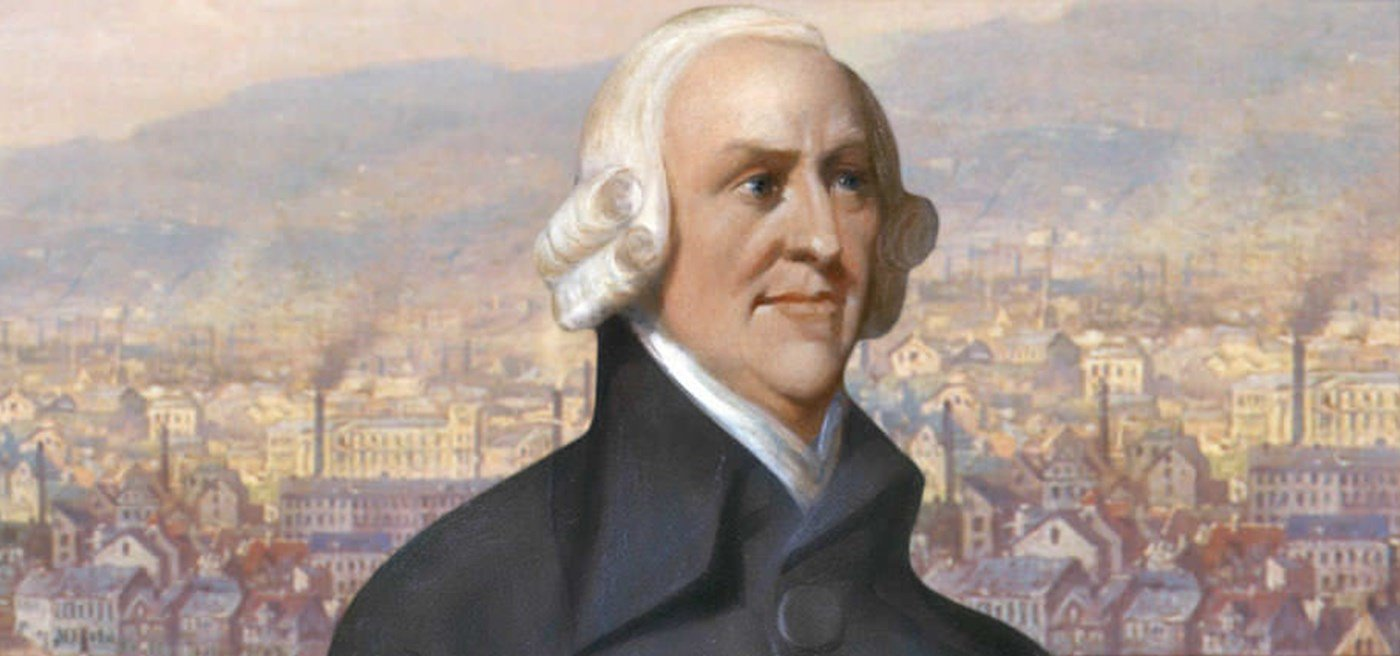
\includegraphics[width=5cm]{./IO_Week2_Smith.jpg}}
\end{picture}

\bi
\item Adam Smith offers the first story
\item Claim: Firms exist to enable specialization 
\item Story 1: People's minds are more erfficient when focused
\item Story 2: There are switching costs between tasks
\item Limitation: Explains why there is specialization, not why firms exist
\ei

}


\frame{\ft{Theory of the firm 2: Risk aversion}

\setbeamertemplate{itemize items}[triangle]

\begin{picture}(80,80)(0,0) %syntax: \begin{picture}(width,height)(x-offset,y-offset)
\put(240,-20){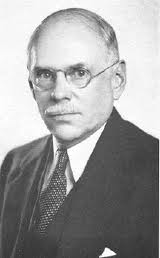
\includegraphics[width=3cm]{./IO_Week2_Knight.jpg}}
\end{picture}

\bi
\item Frank Knight offers a second solution
\item Claim: Variation in forecasting ability
\item Story: Some people can forecast demand, they hire people to help them react to their own forecast. Since the others can't trust the forecaster, they demand compensation that does not depend on performance. 
\item Limitation: Doesn't explain why there are firms even when demand is easier to forecast. 
\item Plausible revision: Variance in risk aversion
\ei

}

\frame{\ft{Theory of the firm 3: Transaction costs}

\setbeamertemplate{itemize items}[triangle]

\begin{picture}(80,80)(0,0) %syntax: \begin{picture}(width,height)(x-offset,y-offset)
\put(240,-20){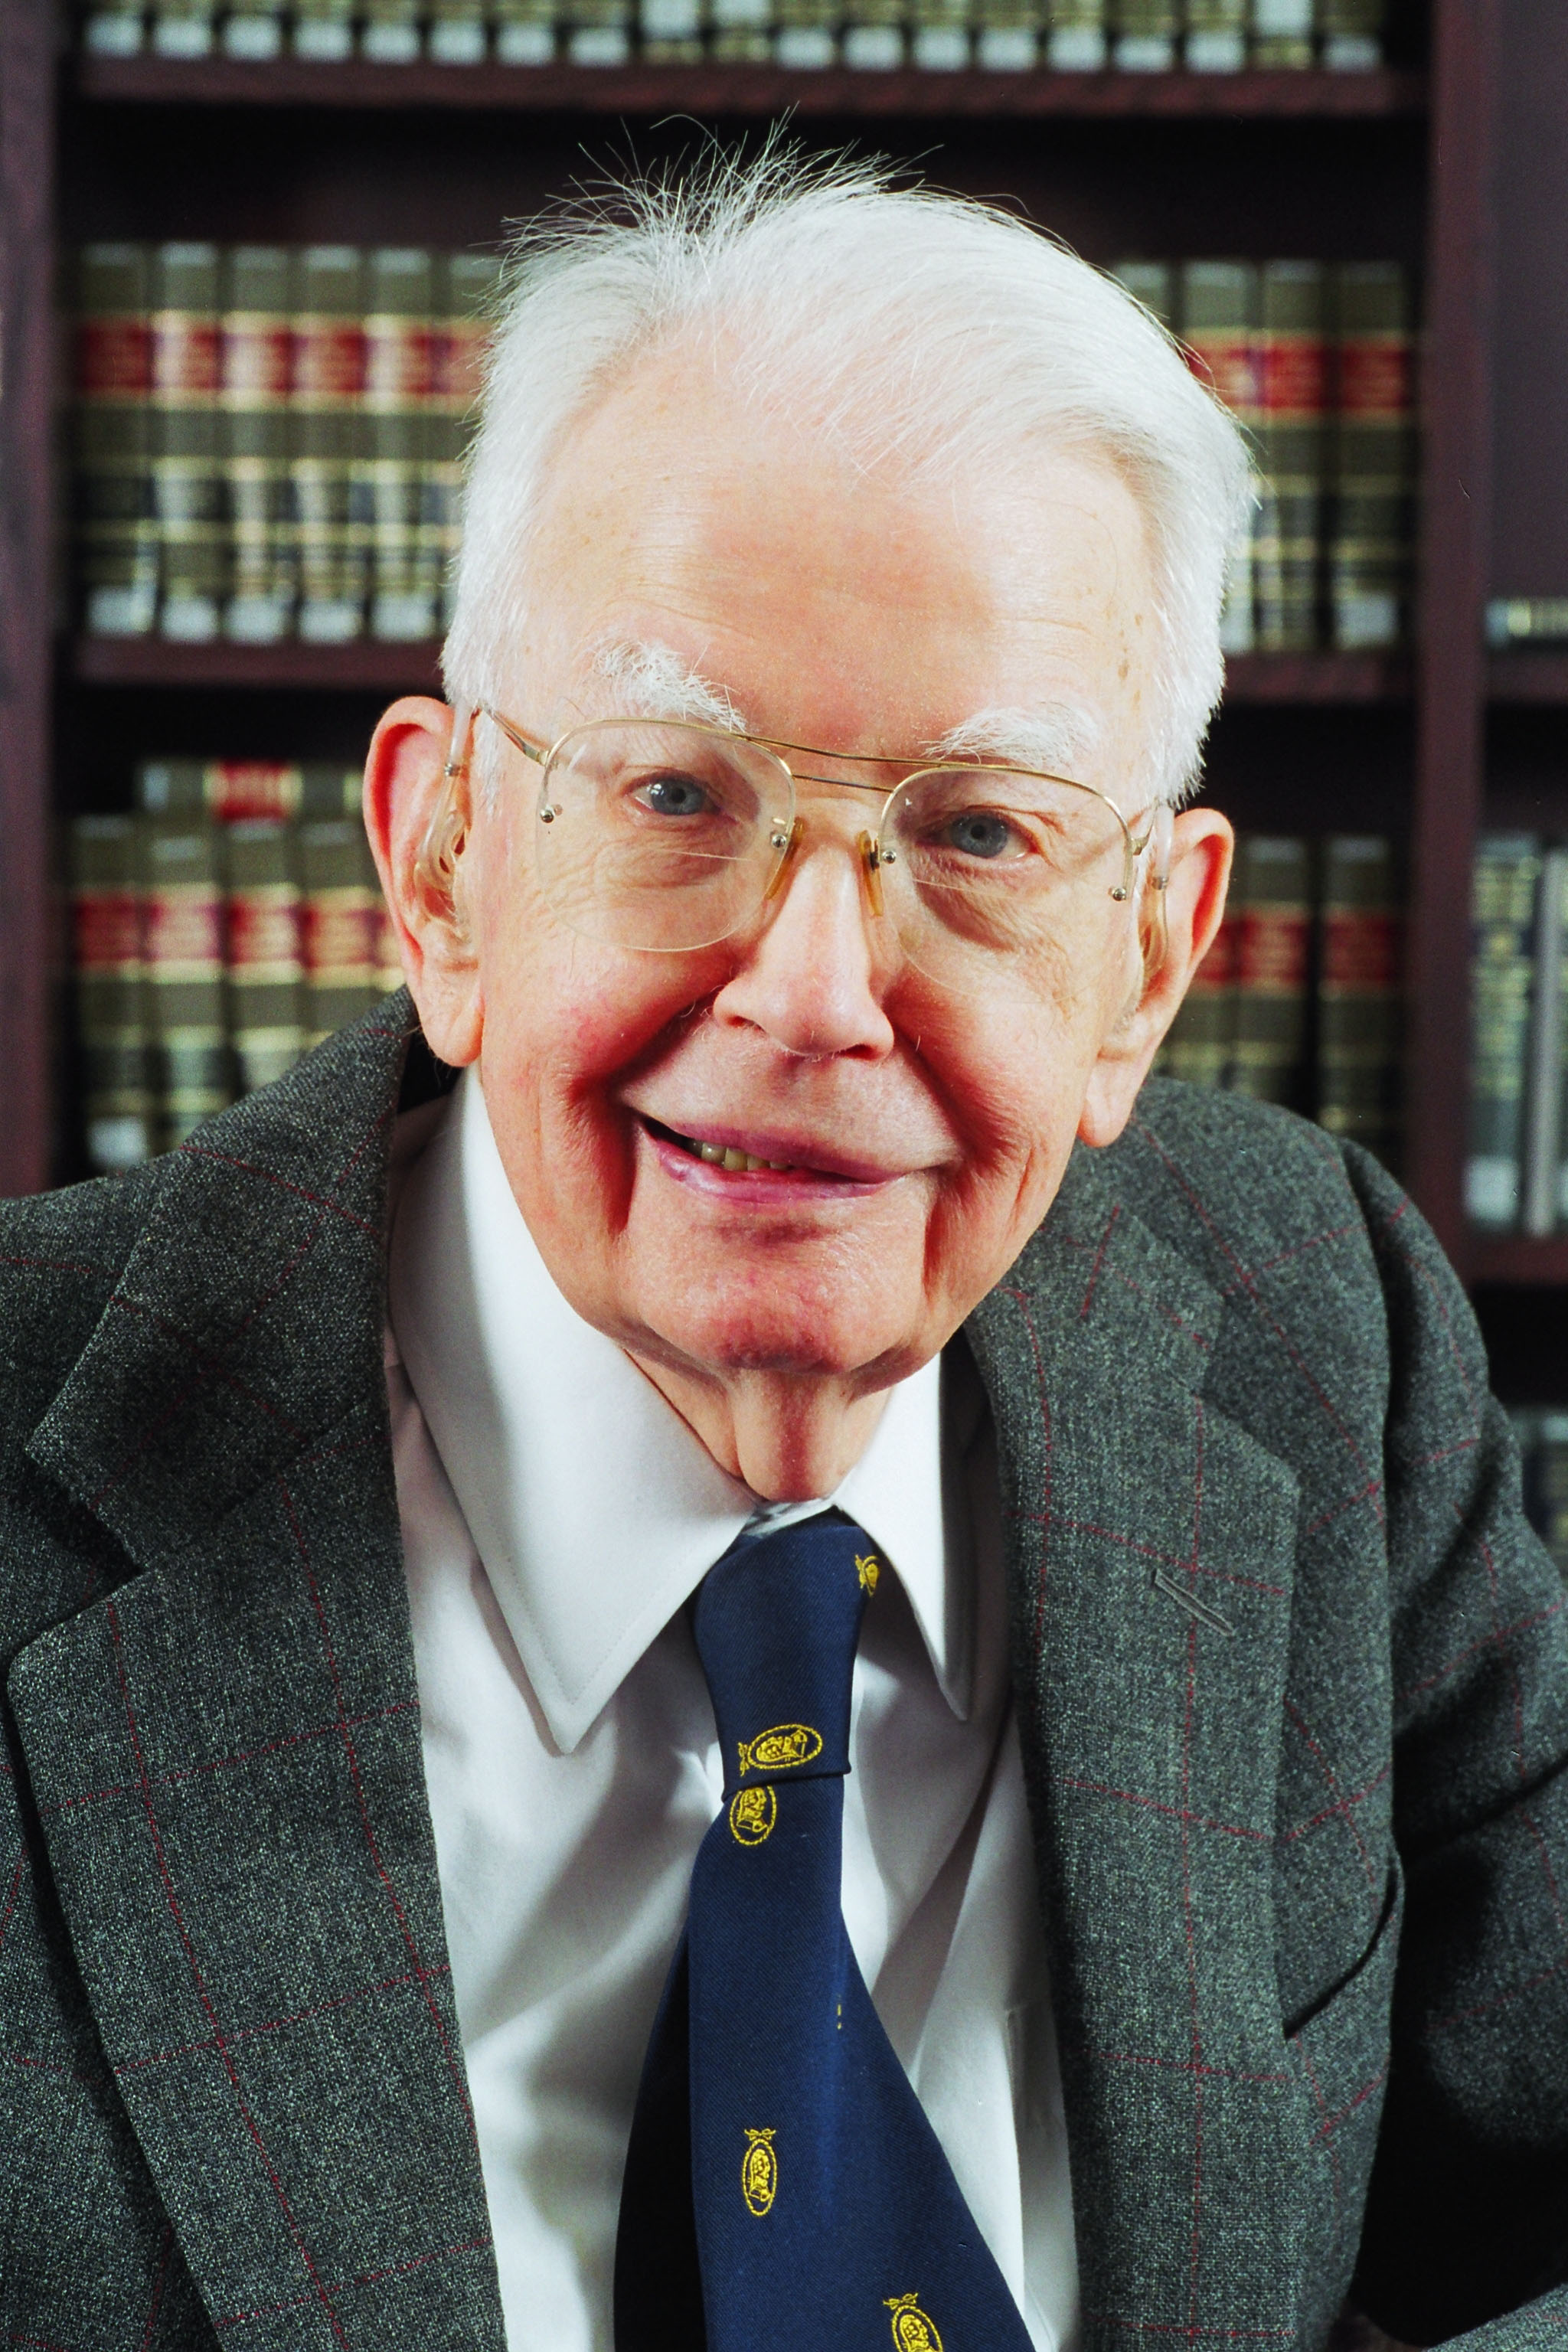
\includegraphics[width=3cm]{./IO_Week2_Coase.jpg}}
\end{picture}

\bi
\item Coase, seminal "Nature of the firm"
\item Claim: Presence of transaction costs
\item Story: Firms exist because there is a cost to using the market price
\item Limitation: Moves the question to, why are there transaction costs?
\ei

}

\frame{\ft{Theory of the firm 3: Transaction costs}

\setbeamertemplate{itemize items}[triangle]


Consider a rancher and farmer. The rancher can consider whether or not to take an action. If he takes the action he benefits to the extent of X but he costs the farmer Y. So clearly the action is beneficial if $X>Y$. But what if there is some cost to the two getting on the table, whatever its nature, psychological, informational, transportation cost etc, then the transaction won't take place at all. The cost of using the price mechanism. 

}


\frame{\ft{Theory of the firm 4: Property rights}

\setbeamertemplate{itemize items}[triangle]

\begin{picture}(80,80)(0,0) %syntax: \begin{picture}(width,height)(x-offset,y-offset)
\put(240,-20){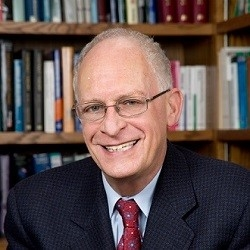
\includegraphics[width=5cm]{./IO_Week2_Hart.jpg}}
\end{picture}

\bi
\item Hart and Moore, Incomplete contracts
\item To form coalitions where ex-ante investment can be rewarded
\item Story: A firm is a structure which has the ability to reward people for things they didn't contract for. 
\item Limitation: A bit abstract, not clear what it's scope is
\ei

}

% So a firm is defined by a relationship where one party is paid, not via unit, but via time. 

% Does transparency increase or decrease salaries? Why would an employer pay you MORE when he cannot link the outcome to your action? 

% Traditionally, the theory of the firm of Schumpeter, was that firms exist because of specialization. 

% But what is specialization? People perform tasks more efficiently when their mind is focused on one thing. (Learning by doing). 2) Switching costs

% The coasian theorem is a theory of the firm theorem. You vertically integrate when there are transaction costs.
% Consider a rancher and farmer. The rancher can consider whether or not to take an action. If he takes the action he benefits to the extent of X but he costs the farmer Y. So clearly the action is beneficial if X>Y. But what if there is some cost to the two getting on the table, whatever its nature, psychological, informational, transportation cost etc, then the transaction won't take place at all. The cost of using the price mechanism. 

% Take the simplest example. Every year a coin gets flipped and does either +0 or +1 to the owners profits. The manager first SEEs the noise and then chooses whether to work or not. Similarly, his manager can choose either to work or be lazy. Working costs him 0 cents but adds 1 to the owner. The owner can only see a series of number floating (0,2,1,1,1,1,2,0). He knows from the 2 that the manager worked hard and knows from the 0 that he didn't work hard. So how much should he compensate him? 

% Consider the policy (0,50+epsilon,50+epsilon).  The Manager knows that he can slack off and get 50+ epsilon. Whilst if he works hard, he gets only epsilon. So he prefers to simply slack off. On the other hand if the coin flip is 0, if he works he gets epsilon, whilst if he slacks off he gets 0. So We need to motivate him to work when the flip is 0. (0,50+epsilon,100+2epsilon).

% So if the owner, can perfectly monitor the manager, then ONLY then only individual rationality plays a role. If the manager is risk averse, we also get that the salary is independent of the profits. 

\section{Monopoly}

\frame{\ft{What is a monopoly}

\setbeamertemplate{itemize items}[triangle]

\bi
\item What is a monopoly?
\item Definition: When there is only a single seller
\item Why does it emerge?
\item Natural monopoly, Government privileges, Historic reasons, Reputations
\item Effect of monopoly:
\item It reduces the quantity sold and increases prices. Unless it can discriminate, 
\item If monopolist can perfectly discrminate, first best, perfect appropriation
\ei

}

\frame{\ft{The firm: Revenue}

\setbeamertemplate{itemize items}[triangle]

\begin{align*}
Revenue:  R& = p(q)q \\
\text{Marginal Revenue}: MR& = \dfrac{dR}{dq} = \dfrac{dp}{dq}q+p = p(1-\dfrac{1}{\eta}) \\
\text{Where:} \eta & = -\frac{dq}{dp}\frac{p}{q}
\end{align*}

}

\frame{\ft{The firm: Profit}

\setbeamertemplate{itemize items}[triangle]


\begin{align*}
&Profit: max_q \pi(q) = qP(q)-C(q) &\text{Profit as a function of quantity}\\
&FOC: qP'(q)+P(q)-C'(q) = 0  &\text{A positive first derivative at zero is neccesary} \\
&SOC: qP''(q)+2 P'(q)-C''(q)<0  & \text{Unique solution requires negative second derivative}\\
& \text{Lerner's index}:  \frac{P(q)-C'(q)}{P(q)}= \dfrac{1}{\eta} & \text{FOC re-arranged and divide by P} \\
\end{align*}
\text{So the monopolist increases his markup as the demand becomes less price elastic}

}

\frame{\ft{Monopoly Graph}

\setbeamertemplate{itemize items}[triangle]


\begin{picture}(80,80)(0,0) %syntax: \begin{picture}(width,height)(x-offset,y-offset)
\put(0,-100){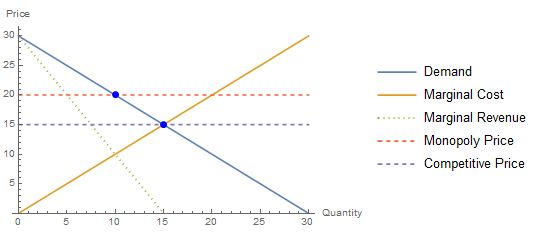
\includegraphics[width=15cm]{./IO_Week2_Monopoly.jpg}}
\end{picture}

}

% Now with that caveat in mind, let's dig into the profit of the firm. 

% Let's take the simplest case: 
% $max_q \pi(q) = qP(q)-C(q)$
% $qP'(q)+P(q)-C'(q)$
% 
% 
% $P(q)-C'(q)/P(q)=1/ \ita$

% So the monopolist increases his markup as the demand becomes less price elastic. 


\end{document}